\documentclass{article}
\usepackage[utf8]{inputenc}
\usepackage[spanish,mexico]{babel}
\usepackage[a4paper,top=1.5cm,bottom=1.5cm,left=2cm,right=2cm]{geometry}
\usepackage{caption,subcaption}
\usepackage{amsmath}
\usepackage{cancel}
\usepackage{natbib}
\title{Turbiedad}
\author{Lalih Otrebor feat. Cana Inalec}
\date{April 2019}
\usepackage{siunitx}
\usepackage{graphicx}
\usepackage{bm}

\newcommand{\glossentry}[2]{$#1$\indent #2 \par \vspace{.4cm} }


%
\newcommand{\tita}{\theta}
\newcommand{\substy}[2]{\ensuremath{{#1_{\mathrm{#2}}}}}
\newcommand{\sib}[1]{\ensuremath{\left[\si{#1}\right]}}
\newcommand{\degree}{\ensuremath{{^\circ}}}
\newcommand{\attackangle}{{\ensuremath{\bm{\alpha}}}}
\newcommand{\cp}{c_p}
\newcommand{\cteuniversal}{\ensuremath{\tilde{R}}}
\newcommand{\molarmass}{\ensuremath{{\scriptstyle \bar{M}}}}
\newcommand{\Rconst}{R}
\newcommand{\gasconst}{k}
\newcommand{\ctegas}{\gasconst}
% \newcommand{\speedsound}{{c_{\!s\!}}}
\newcommand{\relative}{\mathrm{rel}}
\newcommand{\speedsound}{a}
\newcommand{\ctan}[1]{\ensuremath{c_{\theta #1}}}
\newcommand{\crad}[1]{\ensuremath{c_{r #1}}}
\newcommand{\cax}[1]{\ensuremath{c_{a #1}}}
\newcommand{\angvel}{\ensuremath{\omega}}
\newcommand{\Mach}{\textrm{M}}
\newcommand{\di}{\textrm{d}}
\newcommand{\cte}{\textrm{constante}}
%Entradas para glosario 
\newcommand{\etaiso}{\eta_{\mathrm{iso}}}
\newcommand{\Sgen}{\substy{S}{gen}}
\newcommand{\dQ}{\dot{Q}}
\newcommand{\dW}{\dot{W}}
\newcommand{\dm}{\dot{m}}
\newcommand{\etaTot}{\substy{\eta}{iso}}
\newcommand{\etahid}{\substy{\eta}{h}}
\newcommand{\etamec}{\substy{\eta}{m}}
\newcommand{\slip}{\xi}
\newcommand{\slipangle}{\ensuremath{\theta_d}}
\newcommand{\radrel}{\nu}
\newcommand{\rext}{\substy{r}{ext}}
\newcommand{\rbase}{\substy{r}{base}}
\newcommand{\powerreduction}{\mu}
\newcommand{\degreeofreaction}{{\bm{R}}}
\newcommand{\relcomp}{\ensuremath{r_c}}
\begin{document}

\maketitle

\section*{Glosario}
Subíndice $1$ indica la entrada al rotor, $2$ indica salida del rotor, $B_s$ indica el estado $B$ para el proceso isoentrópico.
\par

\glossentry{\speedsound}{La velocidad del sonido en un fluido}


\glossentry{c}{Velocidad absoluta del fluido}
% \glossentry{\cax{}=V}{Velocidad axial del fluido}
\glossentry{\ctan{}}{Velocidad tangencial del fluido}
\glossentry{\cax{}}{Velocidad axial del fluido}

\glossentry{\crad{}}{Velocidad radial del fluido}
\glossentry{w}{Velocidad relativa del fluido con respecto al rotor}
\glossentry{U}{Velocidad del impulsor}
\glossentry{\cteuniversal=8,314 \si{\joule \per \kelvin\per \mole}}{Constante universal para gases ideales}
\glossentry{R=\molarmass\cteuniversal}{Constante especifica de un gas ideal \sib{\joule \per \kilogram \per \kelvin} donde \molarmass{} es la masa molar \sib{\kilogram \per \mole}}
\glossentry{\degreeofreaction}{Grado de reacción}
\glossentry{\relcomp}{Relación de compresión}
\glossentry{r,D}{Radio y diámetro, respectivamente}
\glossentry{\Mach=\frac{c}{\speedsound}}{Número de Mach}
\glossentry{\alpha}{Ángulo entre velocidad absoluta con respecto al plano meridional}
\glossentry{\attackangle}{Ángulo de ataque del alabe}
\glossentry{\beta}{Ángulo entre velocidad relativa con respecto al plano meridional}
\glossentry{\delta}{Ángulo de desviación del alabe o espesor de capa límite}
% \glossentry{\slipangle}{Ángulo de deslizamiento}
\glossentry{\psi}{Coeficiente}
\glossentry{\phi}{Coeficiente de flujo $\frac{\crad{2}}{U_2}$}
\glossentry{\slip}{Coeficiente de deslizamiento}
\glossentry{\Omega}{Velocidad angular del rotor}



% end of glossary
%------------------
\section{Ecuaciones de gas compresible}
Definimos $\cteuniversal=8,314$ \si{\joule \per \kelvin\per \mole} como la constante universal de gases tal que $\cteuniversal = \frac{R}{\molarmass}$ donde $\molarmass$ es la masa molar.
\begin{figure}[htb!]
\centering
\begin{subfigure}{.49\textwidth}
\centering
\includegraphics[height=6cm]{fig/caracteristicascompresor.png}
\caption{Compresor}
\label{fig:caractcompresor}
\end{subfigure}%
\begin{subfigure}{.49\textwidth}
\centering
\includegraphics[height= 6cm]{fig/caracteristicasturbina.png}
\caption{Turbina}
\label{fig:caractturbina}
\end{subfigure}
\caption{Características de turbomáquinas.}
\label{fig:caracteristicasturbomaquinas}
\end{figure}
\subsection{Entalpía de estancamiento} 
Constante para un proceso que no involucra transferencia de trabajo o transferencia de calor aunque si pueden estar presentes procesos irreversibles.
\[
h_0 = h+\tfrac{1}{2}c^2
\]
si el fluido es gas perfecto \( h=\cp T\) donde \( \cp = \gasconst \Rconst (\gasconst-1)^{-1} \).
\[
T_0 = T + \tfrac{1}{2}\frac{c^2}{\cp}
\]

\begin{equation}\label{eq:tempstagnation}
 \frac{T_0}{T}=1+\tfrac{1}{2}(\gasconst-1)\frac{c^2}{\gasconst\Rconst T}=1+\tfrac{1}{2}(\gasconst-1)\Mach^2
\end{equation}
La relación de Gibbs derivada de la segunda ley:
\[T\di s = \di h - \frac{1}{\rho}\di p
\]
si el fluido es traído al reposo mediante un proceso adiabático y reversible entonces

\[\di h = \cp \di T =\frac{\di p}{p}\Rconst T
\]
tal que
\[
\frac{\di p}{p} = \frac{\cp}{\Rconst}\frac{\di T}{T} = \frac{\gasconst}{\gasconst-1}\frac{\di T}{T}
\]
integrando obtenemos
\[
\ln p = \ln \cte + \frac{\gasconst}{\gasconst-1}\ln T
\]
por ende
\begin{equation}
    \frac{p_0}{p}=\left(\frac{T_0}{T} \right)^{\frac{\gasconst}{\gasconst-1}} =\left(1+ \frac{\gasconst-1}{2}\Mach^2 \right)^{\frac{\gasconst}{\gasconst-1}}
\end{equation}
y de la ley de gases ideales sabiendo que \(\rho = p/(RT)=\frac{1}{v} \)


\begin{equation}
    \frac{\rho_0}{\rho}=\left(\frac{T_0}{T} \right)^{\frac{1}{\gasconst-1}} =\left(1+ \frac{\gasconst-1}{2}\Mach^2 \right)^{\frac{1}{\gasconst-1}}
\end{equation}
\[
\Mach=\frac{c}{\speedsound} = \frac{c}{\sqrt{\gasconst \Rconst T}}
\]
\subsection{Ecuaciones de Euler para bombas y turbinas}

La ecuación de Euler es un modelo para el torque y la potencia de una turbomáquina. Utiliza el flujo másico, la velocidad angular y la geometría. Se obtiene a partir de la conservación de momento angular. 

\subsection*{Triángulo de velocidades} Para el estudio del flujo en el interior de una turbomáquina se define la velocidad de flujo $\Vec{c}$ absoluta, la velocidad de flujo relativa $\Vec{w}$ y la velocidad del sistema móvil $\Vec{U}=\Omega \times r$ y los ángulos $\alpha$, $\beta$ y $\theta$. Los distintos libros usan distintas letras para los ángulos, lo que hace que las ecuaciones se vean distintas. Aquí se toman los nombres usados por Dixon, que figura en \ref{fig:veltrianggeneral}. 

El triángulo de velocidades no es más que la aplicación de los principios de mecánica General: 

\[\Vec{c}=\Vec{U}+\Vec{w}\]

Parado en el sistema móvil, donde las paletas están fijas, se observaría que el flujo es tangente a la paleta. Por eso en los triángulos de velocidades se debe dibujar $\Vec{w}$ en esa dirección. Quedan relacionadas las velocidades con los ángulos de ataque y de fuga del diseño.  

\subsubsection*{Continuidad o Conservación de la masa}
Si el enunciado no informa acerca de las velocidades, éstas se pueden relacionar con el flujo másico teniendo en cuenta que la materia que ingresa es la misma que la que sale (tanto en el sistema absoluto como en el móvil).

la ecuación tiene la forma de 
\[
\dm=\rho_1 A_1 c_{n1} = \rho_2 A_2 c_{n2}
\]

donde $c_{ni}$ es la velocidad del fluido en dirección normal a la superficie de área $A_i$. En turbinas axiales la velocidad $c_{n}$ no es otra que $c_{a}$, y se suele constante en el álabe porque el cambio de densidad no es pronunciado. 
\subsubsection{Conservación de la cantidad de momento angular}
\begin{figure}[htb!]
    \centering
    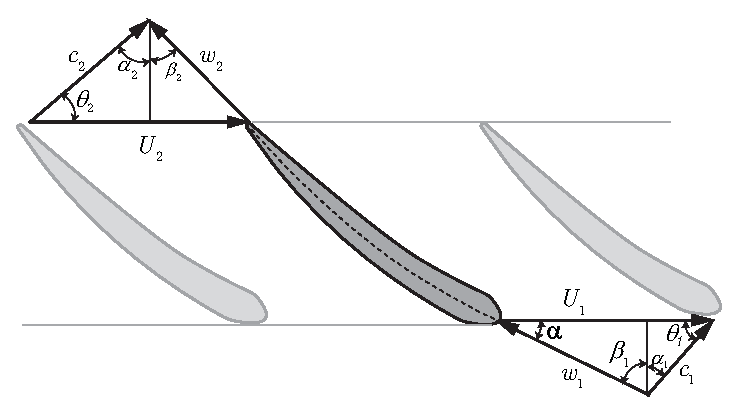
\includegraphics[width=0.6\textwidth]{fig/VelTrianglegeneral.eps}
    \caption{Triangulo de velocidades para un alabe de un rotor de un compresor axial. Gira en sentido de $U$.}
    \label{fig:veltrianggeneral}
\end{figure}


\begin{figure}
    \centering
    \includegraphics[width=9cm]{fig/turb.png}
    \caption{$\Omega=\angvel,\quad$      $\tau_A=\dot{m}(r_2 \ctan{2} -r_1 \ctan{1}$)}
    \label{fig:turbina}
\end{figure}

Al aplicar la conservación de momento angular se obtiene la ecuación de Euler. Recordar que $\Omega \tau = \dW$ es la potencia intercambiada.

\begin{equation}\label{eq:eulerparaTubomaquinas}
    \tau= \dot{m} (r_2\ctan{2} -r_1 \ctan{1})  \quad \Rightarrow\quad \dW =\dm (U_2 c_2 \cos \theta_2 - U_1 c_1 \cos \theta_1)  
\end{equation}

Una de las consecuencias útiles es que si se aplica el teorema del coseno a la figura \ref{fig:veltrianggeneral} se tiene que

\[
w^2 = U^2 +c^2 -2U c \cos \theta 
\]
por ende tenemos que $Uc \cos \theta = (w^2-U^2-c^2)/2$, resultando en la ecuaci'on expandida de Euler \ref{eq:eulerexpanded}

\begin{equation} \label{eq:eulerexpanded}
    \frac{\dot{W}}{\dot{m}}=e=(h_{02}-h_{01})= \left(\frac{c_2^2-c_1^2}{2}\right)+\left(\frac{U_2^2-U_1^2}{2}\right)+\left(\frac{w_1^2-w_2^2}{2}\right)
\end{equation}





\subsection{Segunda Ley -- Entropía}
Por alguna razón (Enunciado de Clausius) establece que para un sistema recorriendo un ciclo

\[
\oint \frac{\di Q}{T} \leq 0
\]
La cantidad que se obtiene con el integral se denomina \textit{entropía}. Para un ciclo reversible dicha integral da cero.

\[
S_2 - S_1 = \int^2_1 \frac{\di Q}{T}
\]

Para un sistema en régimen estacionario
\[
\int^2_1 \frac{\di\dot{Q}}{T} \leq \dot{m}(s_2 -s_1)
\]
si el proceso es adiabático $\di \dot{Q}=0$ entonces $s_2\geq s_1$.  Si el proceso además es reversible también entonces $s_2 =s_1$.

Esto sale de la igualdad de termodinámica
\[
\cancelto{\textrm{Adb.}}{\Delta S_0} + \cancelto{\textrm{Rev.}}{\Delta S} = \cancelto{\textrm{Iso.}}{\Sgen} \geq 0
\]

\section{Definiciones de eficiencias}
Según la primera ley de la termodinámica tenemos que el cambio en la energía interna esta dada por
\begin{equation}
    \dot{U} =\dQ -\dW = \dm \left[(h_2-h_1)+\tfrac{1}{2}(c_2^2-c_1^2)+g(z_2-z_1) \right]
\end{equation}
Como la mayoría de las turbomáquinas se aproximan a ser adiabáticas y que los cambios en energía potencial son insignificantes en la gran mayoría de los casos llegamos a
\begin{equation}
    \dW = \dm \left[ h_1+\tfrac{1}{2}c_1^2 - (h_2+\tfrac{1}{2}c_2^2) \right] = \dm \left( h_{01}-h_{02}\right)
\end{equation}

para compresores (absorben energía) es más conveniente escribir
\[
\dW_c=-\dW =\dm \left( h_{02}-h_{01}\right)
\]

Un trayecto sin intercambio de trabajo para flujos incompresibles y flujos compresibles isoentrópico la presión de estancamiento es constante
\[
p_{01}=p_{02}=p_0=\cte
\]
$p_0$ siendo la presión de estancamiento $p_{0}=p+\tfrac{1}{2} \rho c^{2}$.
\subsection{Eficiencia}
La eficiencia total:
\[
\etaTot  = \frac{\textrm{Potencia mecánica disponible a la salida del eje}}{\textrm{Máxima diferencia de energía posible en el fluido por unidad tiempo}}
\]
LA eficiencia isotentrópica o hidraulica:
\[
\etaiso=\etahid = \frac{\textrm{Potencia mecánica suministrada al rotor}}{\textrm{Máxima diferencia de energía posible en el fluido por unidad tiempo}}
\]
La eficiencia mecánica:
\[
\etamec = \frac{\etaTot}{\etaiso}
\]

Para un flujo incompresible, en la ausencia de fricción se tiene que la potencia máxima que se puede obtener de una turbina es
\[
\dW_{\max} = \dm  \left[ (h_{01}-h_{02s})+g(z_1-z_2) \right]= \dm g \left(H_1-H_2 \right)
\]
donde $gH = \frac{p}{\rho}+\frac{1}{2}c^2+gz$.

\begin{figure}[htb!]
\centering
\begin{subfigure}{.49\textwidth}
\centering
\includegraphics[height=6cm]{fig/expansionturbina.png}
\caption{Proceso de expansión en una turbina}
\label{fig:expansiontrubina}
\end{subfigure}%
\begin{subfigure}{.49\textwidth}
\centering
\includegraphics[height= 6cm]{fig/procesocompresion.png}
\caption{Proceso de compresión }
\label{fig:procesocompresion}
\end{subfigure}
\caption{Diagramas $h$--$s$ para turbinas y compresores}
\label{fig:procesosturbomaquinasHS}
\end{figure}



\section{Compresores centrífugos}


El borde del inductor debe tener el mismo ángulo que tiene la velocidad relativa del fluido ($\beta_1$) al entrar en la bomba y así evitar el choque entre inductor y fluido. Para un fluido sin prerotación:
\[
\tan \beta_1 = \frac{\cax{1}}{U_1}
\]

\subsection{Deslizamiento}
Aún en condiciones ideales con alabes sin fricción el flujo es impulsado de manera imperfecta por los alabes debido a la aceleración de Coriolis. Se dice que el fluido \textit{desliza}. Se podría pensarlo como una diferencia de presión entre las dos superficies de un alabe dando luz a una velocidad relativa en dirección opuesta a la rotación. El efecto aumenta con la luz entre alabes, por ende se necesita un número \textbf{infinito} de alabes para que no haya deslizamiento.

\begin{figure}[htb!]
\centering
\begin{subfigure}{.49\textwidth}
\centering
\includegraphics[height=5cm]{fig/eddydeslizamiento.png}
\caption{Eddy relativa formada por haber finitos alabes}
\label{fig:deslizamientoEddy}
\end{subfigure}%
\begin{subfigure}{.49\textwidth}
\centering
\includegraphics[height= 5cm]{fig/deslizamientoconeddy.png}
\caption{Flujo ideal sumado con eddy}
\label{fig:deslizamientoEddyMasFlujoIdeal}
\end{subfigure}
\caption{Visualización del deslizamiento}
\label{fig:explicaciondeslizamiento}
\end{figure}

\subsection{El coeficiente de deslizamiento}
Todas las velocidades son a la salida del rotor. El coeficiente de deslizamiento:
\[
\slip = \frac{\ctan{d}}{\ctan{}} = \frac{\ctan{}-u_d}{\ctan{}}
\]

Un estimativo de la velocidad de deslizamiento $u_d= \ctan{}-\ctan{\mathrm{deslizando}}$ sale de suponer que los eddys tienen el diámetro igual al espacio entre alabes $D_{\mathrm{eddy}}= \pi D_{\mathrm{2}}/Z$ donde $Z$ es el número de alabes. 
\[
u_d \sim \Omega \cdot \frac{D_{\mathrm{eddy}}}{2}
\]
donde $\ctan{}$ es la velocidad obtenida con la ecuación de Euler que no toma en cuenta el deslizamiento. El ángulo que se desvía el flujo por causa del deslizamiento:
\[
\tan (\beta_d) =\frac{\ctan{}-\ctan{d}}{\crad{}}= \frac{u_d}{\crad{}}
\]

Stodola (1927) propone una correlación para alabes curvos donde $\beta_2$ es el ángulo del alabe a la salida del rotor respecto la radial.

\[
D_{\mathrm{eddy}}\simeq \frac{\pi D_2\cos \beta_2}{Z} \quad\Rightarrow \quad \slip_{\mathrm{Stodola}} = 1-\frac{\pi \cos \beta_2}{Z(1-\phi_2 \tan \beta_2)}
\]
donde $\phi_2 =\frac{\crad{2}}{U_2}$.

Correlación Wiesner--Busemann (1967) (``la mejor", Se aproxima a la realidad):
\[
\ctan{d} =\frac{U_2\sqrt{\cos \beta_2}}{Z^{0,7}}
\quad\Rightarrow\qquad
\slip_{\mathrm{w}} = 1 - \frac{\sqrt{\cos \beta_2}}{Z^{0,7}(1-\phi_2\tan \beta_2)}
\]

\begin{figure}[htb!]
    \centering
    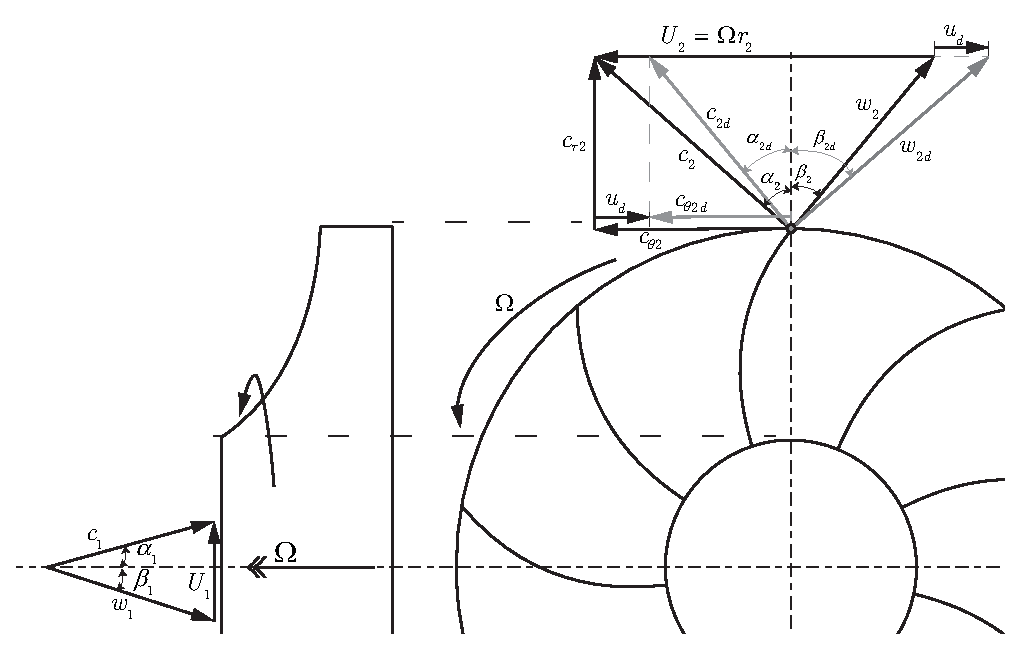
\includegraphics[width=0.7\textwidth]{fig/centrifugoVelocityTriangle.eps}
    \caption{Triángulos de velocidad para una bomba centrifuga con alabes curvados hacia atrás y con pre-rotación $\alpha_1$ positiva. }
    \label{fig:my_label}
\end{figure}
\subsection{Consideraciones del deslizamiento}
Potencia especifica:
\[
\frac{\dW_d}{\dm}=e_d = h_{02}-h_{01}=\ctan{2d} U_2 - \ctan{1} U_1 = (\slip \ctan{2})U_2 - \ctan{1} U_1
\]

\[
T_{03}-T_{01} = \frac{\slip \ctan{2}U_2-\ctan{1}U_1}{\cp}
\]

\[
\etaiso = \frac{\dW_{\mathrm{iso}}}{\dW_{\mathrm{real}}} = \frac{h_{03s}-h_{01}}{h_{03}-h_{01}}= \frac{T_{03s}-T_{01}}{T_{03}-T_{01}}
\]

\[
\frac{p_{03}}{p_{01}}= \left( \frac{T_{03s}}{T_{01}}\right)^{\frac{\ctegas}{\ctegas-1}} =\left[ 1+ \frac{\etaiso (\slip \ctan{2}U_2 - \ctan{1}U_1)}{\cp T_{01}} \right]
\]

Según valores experimentales el número de Mach ($\Mach$) no puede superar $0,9$ en el inductor. Para una entrada netamente positiva:
\[
\Mach_1 = \frac{\cax{1}}{\speedsound} = \frac{\cax{1}}{\sqrt{\ctegas R T_1}}
\]

En la salida del rotor se permite que el número de Mach sea similar a 1. Suele ser buena practica limitar $\crad{2}$ a ser menor a $\speedsound$,
\[
\Mach_2 = \frac{c_{2d}}{\sqrt{Z_2\ctegas R T_2}}
\]
donde $Z_2$ es el factor de compresibilidad del gas.


\subsection{Difusor}
\newcommand{\equis}{{\ensuremath{x}}}
Conservación de la cantidad de movimiento angular especifica para un punto \equis{} del difusor 
\[
\ctan{2} r_2 = c_2 r_2 \sin \alpha_2= c_\equis r_\equis \sin \alpha_\equis  = \cte
\]
por conservación de la masa
\[
\dm = \rho_2 A_2 \crad{2}  = (2\pi r_2 b_2 )(c_2 \cos \alpha_2) \rho_2 = (2\pi r_\equis b_\equis )(c_\equis \cos \alpha_\equis) \rho_\equis =\cte 
\]
donde $b_2$ es el alto de la salida del rotor. Nos  queda que $\tan \alpha_\equis=\cte$ para un fluido \textit{incompresible}, $\rho_\equis = \cte$.
\subsection{Análisis dimensional para compresores dinámicos}
Dos turbomáquinas son dinámicamente semejantes cuando el vector velocidad es geométricamente similar o paralelo en todos los puntos y con módulos proporcionales.
\begin{align}
    \pi_1 &= \frac{p_{02}}{p_{01}}\\
    \pi_2 &= \dm\frac{\sqrt{R T_{01}}}{D^2 P_{01}}\\
    \pi_3 &= \frac{\Omega}{\sqrt{RT_{01}}}\\
    \pi_4 &= \etaTot
\end{align}

\section{Compresores Axiales}
Se define la relación de radios

\[
\radrel = \frac{\rext}{\rbase}
\]

Se tiene que $U_1=U_2=U$ a lo largo del alabe. Además se diseñan para que la velocidad axial sea constante $\cax{1}=\cax{2}=\cax{}$. con estas hipótesis:
\[
\frac{\dW}{\dm}=U \cax{} (\cos \beta_2 - \cos \beta 1 )
\]

Un escalonamiento entre entrada al rotor y salida del estator nos dará un aumento de presión. Si se puede considerar que la densidad permanece constante (es razonable dado que el incremento en presión suele ser muy reducido en turbocompresores axiales) entonces el proceso es isoentrópico
\[
T\di s = \di h - v \di p =0\quad \Rightarrow \quad h_3 - h_1 = \frac{p_3-p_1}{\rho}
\]

Factor diminución de potencia
\[
\powerreduction = \frac{\Delta \substy{T}{real}}{\Delta \substy{T}{euler}} \quad \text{tal que} \quad \substy{\dW}{real} = \powerreduction \dW
\]

\[
\frac{p_{03}}{p_{01}} = \left[1 + \frac{\etaiso \powerreduction}{\cp T_{01}}U \cax{} (\cos \beta_2 - \cos \beta_1) \right]^{\frac{\ctegas}{\ctegas-1}}
\]
grado de reacción:
\[
\degreeofreaction = \frac{h_2 - h_1}{h_3 - h_1}
\]
en caso de $\rho = \cte$ se convierte en el salto de presiones entre rotor y estator.
\begin{figure}[htb!]
    \centering
    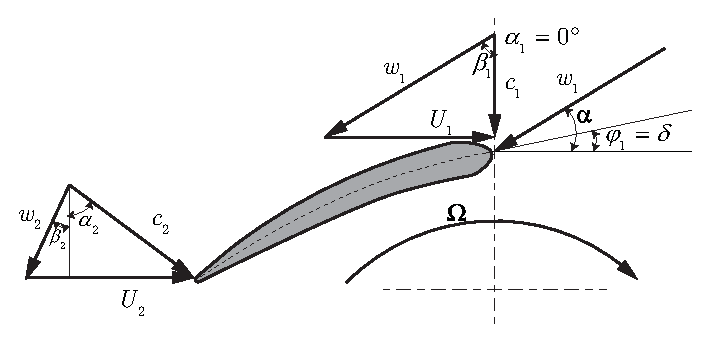
\includegraphics{fig/pumpVelTriangle.eps}
    \caption{Triangulo de velocidades para rotor de compresor axial con velocidad de entrada netamente axial $\alpha_1 = 0\degree$. Nomenclatura de \cite{book:TurboDick} }
    \label{fig:velocitytrianglepump}
\end{figure}

\section{Maquinas de deslpazamiento positivo}





\section{Ebullición}







\bibliography{thebib.bib} % Indica archivo
\bibliographystyle{plainnat}
\end{document}
